\lecture{18 Feb.}

Our course is essentially centered around the modern coding theory of polar codes and LDPC codes. The first half will be about polar coding. Here we give an introduction to the motivation of how polar coding was come up with by Erdal Ar{\i}kan, some of the most non-trivial but stunning results are presented and proven later in the course. We will see how generalizations to polar codes and it related topics influence the agenda of our course.

\section{The Origin of Polar Codes} \label{sec:w1_origin_of_polar_code}

Here we shall trace the paths walked by Ar{\i}kan when he first came up with the ideas of polar coding. For more details, one can refer to the paper ``On the Origin of Polar Coding'' written by Ar{\i}kan \cite{Origin_of_Polar}.

Imaging sending two bits $u_1$ and $u_2$ over the following channel:
\begin{figure}[H]
    \centering
    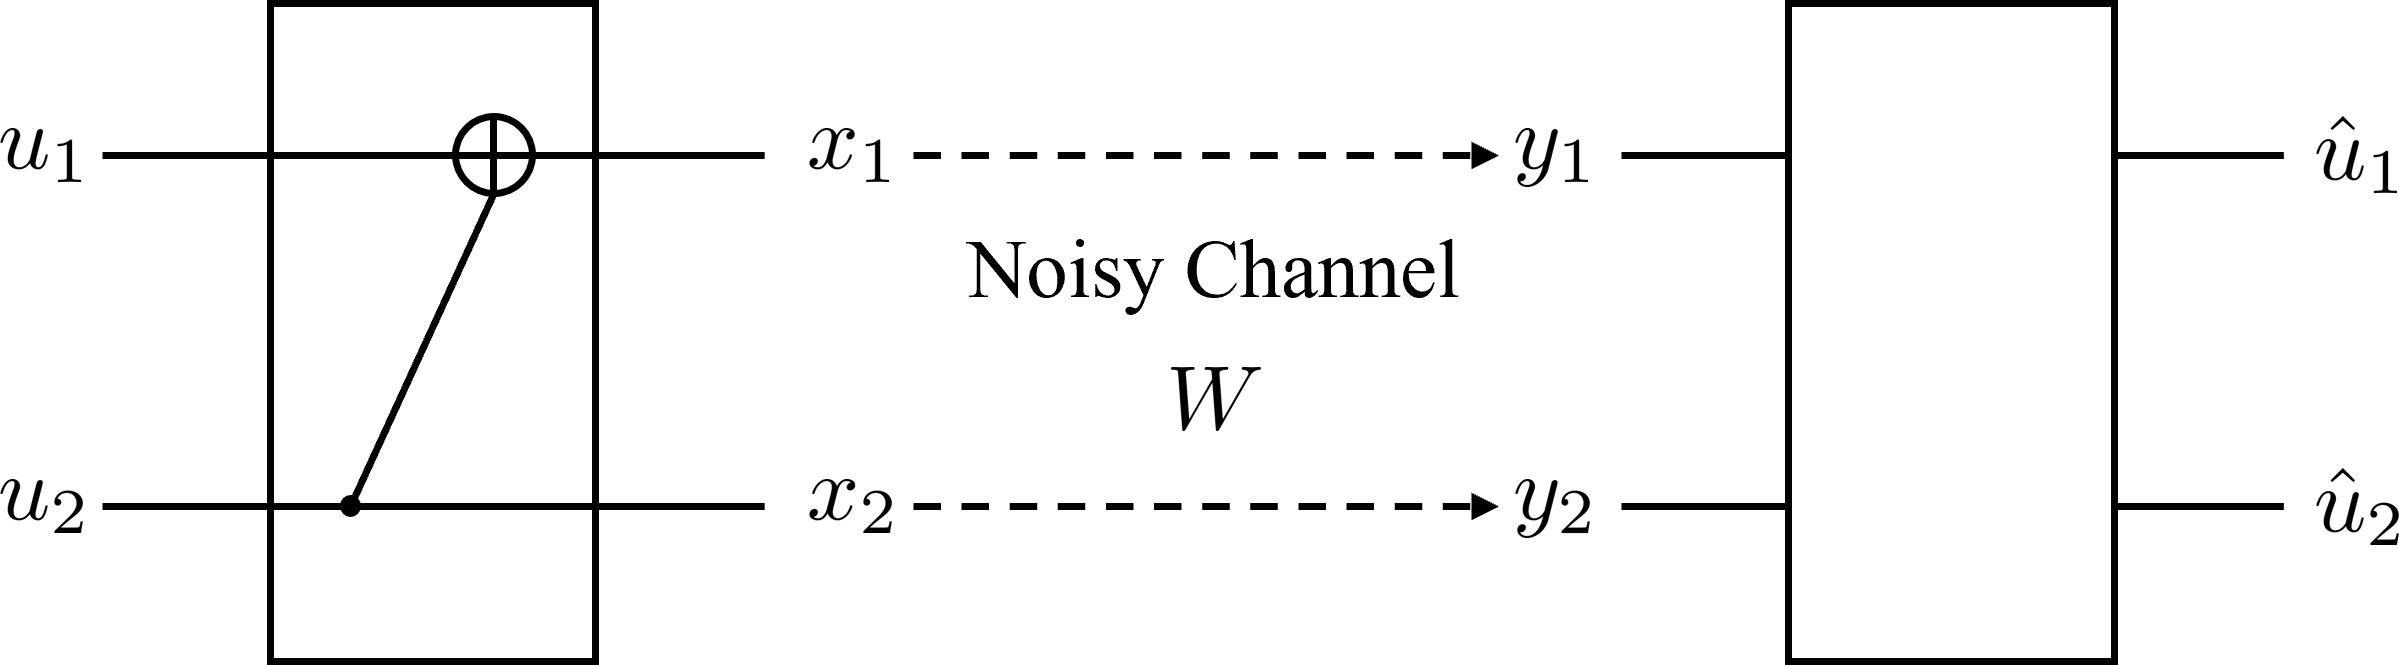
\includegraphics[width=0.7\linewidth]{w1_channel.png}
    \caption{Single-layer polar code.}
    % \label{fig:enter-label}
\end{figure}
We have $y_1$ and $y_2$ being the channel outputs to the channel inputs $x_1=u_1\oplus u_2$ and $x_2=u_2$, respectively, where $\oplus$ is the addition modular 2. If the context is clear, we may write $\oplus$ simply as $+$. If the channel $W$ is faithful, then we can simply set the estimates as $\hat{u}_1 = y_1 \oplus y_2$ and $\hat{u}_2 = y_2$. However, since our channel is noisy, this is simply not the case. What Ar{\i}kan did to construct $\hat{u}_1$ and $\hat{u}_2$ from $y_1$ and $y_2$ was the following procedure:
\begin{enumerate}
    \item Guess $u_1$ by looking at $y_1$ and $y_2$, either via sufficient statistics, or by consensus.
    \item Assume that we did get $u_1$ right, guess $u_2$ by looking at $y_1$, $y_2$, and $u_1$.
\end{enumerate}

What was Ar{\i}kan's motivation for considering the above channel coding scheme? How did he came up with the ``magical'' decoding procedure? First off, one needs to know that his considering of this transformed channel is motivated by the improving of the \textit{cutoff rate} of a channel.

\newpage %formatting

\begin{definition}[Cutoff Rate]
    Given a channel $W:x\rightarrow y$, the cutoff rate is defined as
    \begin{equation}\begin{aligned}
        R_0(W) \defeq&~ \max_{Q\in\Delta(\mathcal{X})}-\lg \sum_{y\in\mathcal{Y}}\left(\sum_{x\in\mathcal{X}}Q(x)\sqrt{W(y\vert x)}\right)^2 \\
        =&~\text{ the rate at which we can communicate ``easily.''}
    \end{aligned}\end{equation}
\end{definition}
Though the mathematical definition of the cutoff rate is fairly complicated, let us only focus on the text description of its purpose: one can immediately tell that $0 < R_0(W) \le C(W)$, where $C(W)=\max_{P_X}I(X;Y)$ is the channel capacity, the theoretical maximum rate for communication over a noisy channel.

Let us denote the whole channel from the bits to the estimates as
\begin{equation}\begin{aligned}
    W^{-} &: u_1 \rightarrow \hat{u}_1, \\
    W^{+} &: u_2 \rightarrow \hat{u}_2.
\end{aligned}\end{equation}
Ar{\i}kan made the following critical observation on the two sub-channels above.

\textbf{Observation}: The cutoff rate of the channel increases:
\begin{equation}
    R_0(W^{-}) + R_0(W^{+}) \ge 2\cdot R_0(W), \label{eq:w1_cutoff_rate_ineq}
\end{equation}
where the inequality is almost always strict.

\begin{remark}
    Note that the capacity remains unchanged:
    \begin{equation}
        C(W^{-}) + C(W^{+}) = 2\cdot C(W).
    \end{equation}
    The equality sign to the cutoff rate inequality \autoref{eq:w1_cutoff_rate_ineq} holds when $W$ is ``extreme'', what is its definition?
\end{remark}

If there is a trick that can increase the cutoff rate \textit{costlessly}, we can do it again and again: an example will be to do it twice, see the figure below.
\begin{figure}[H]
    \centering
    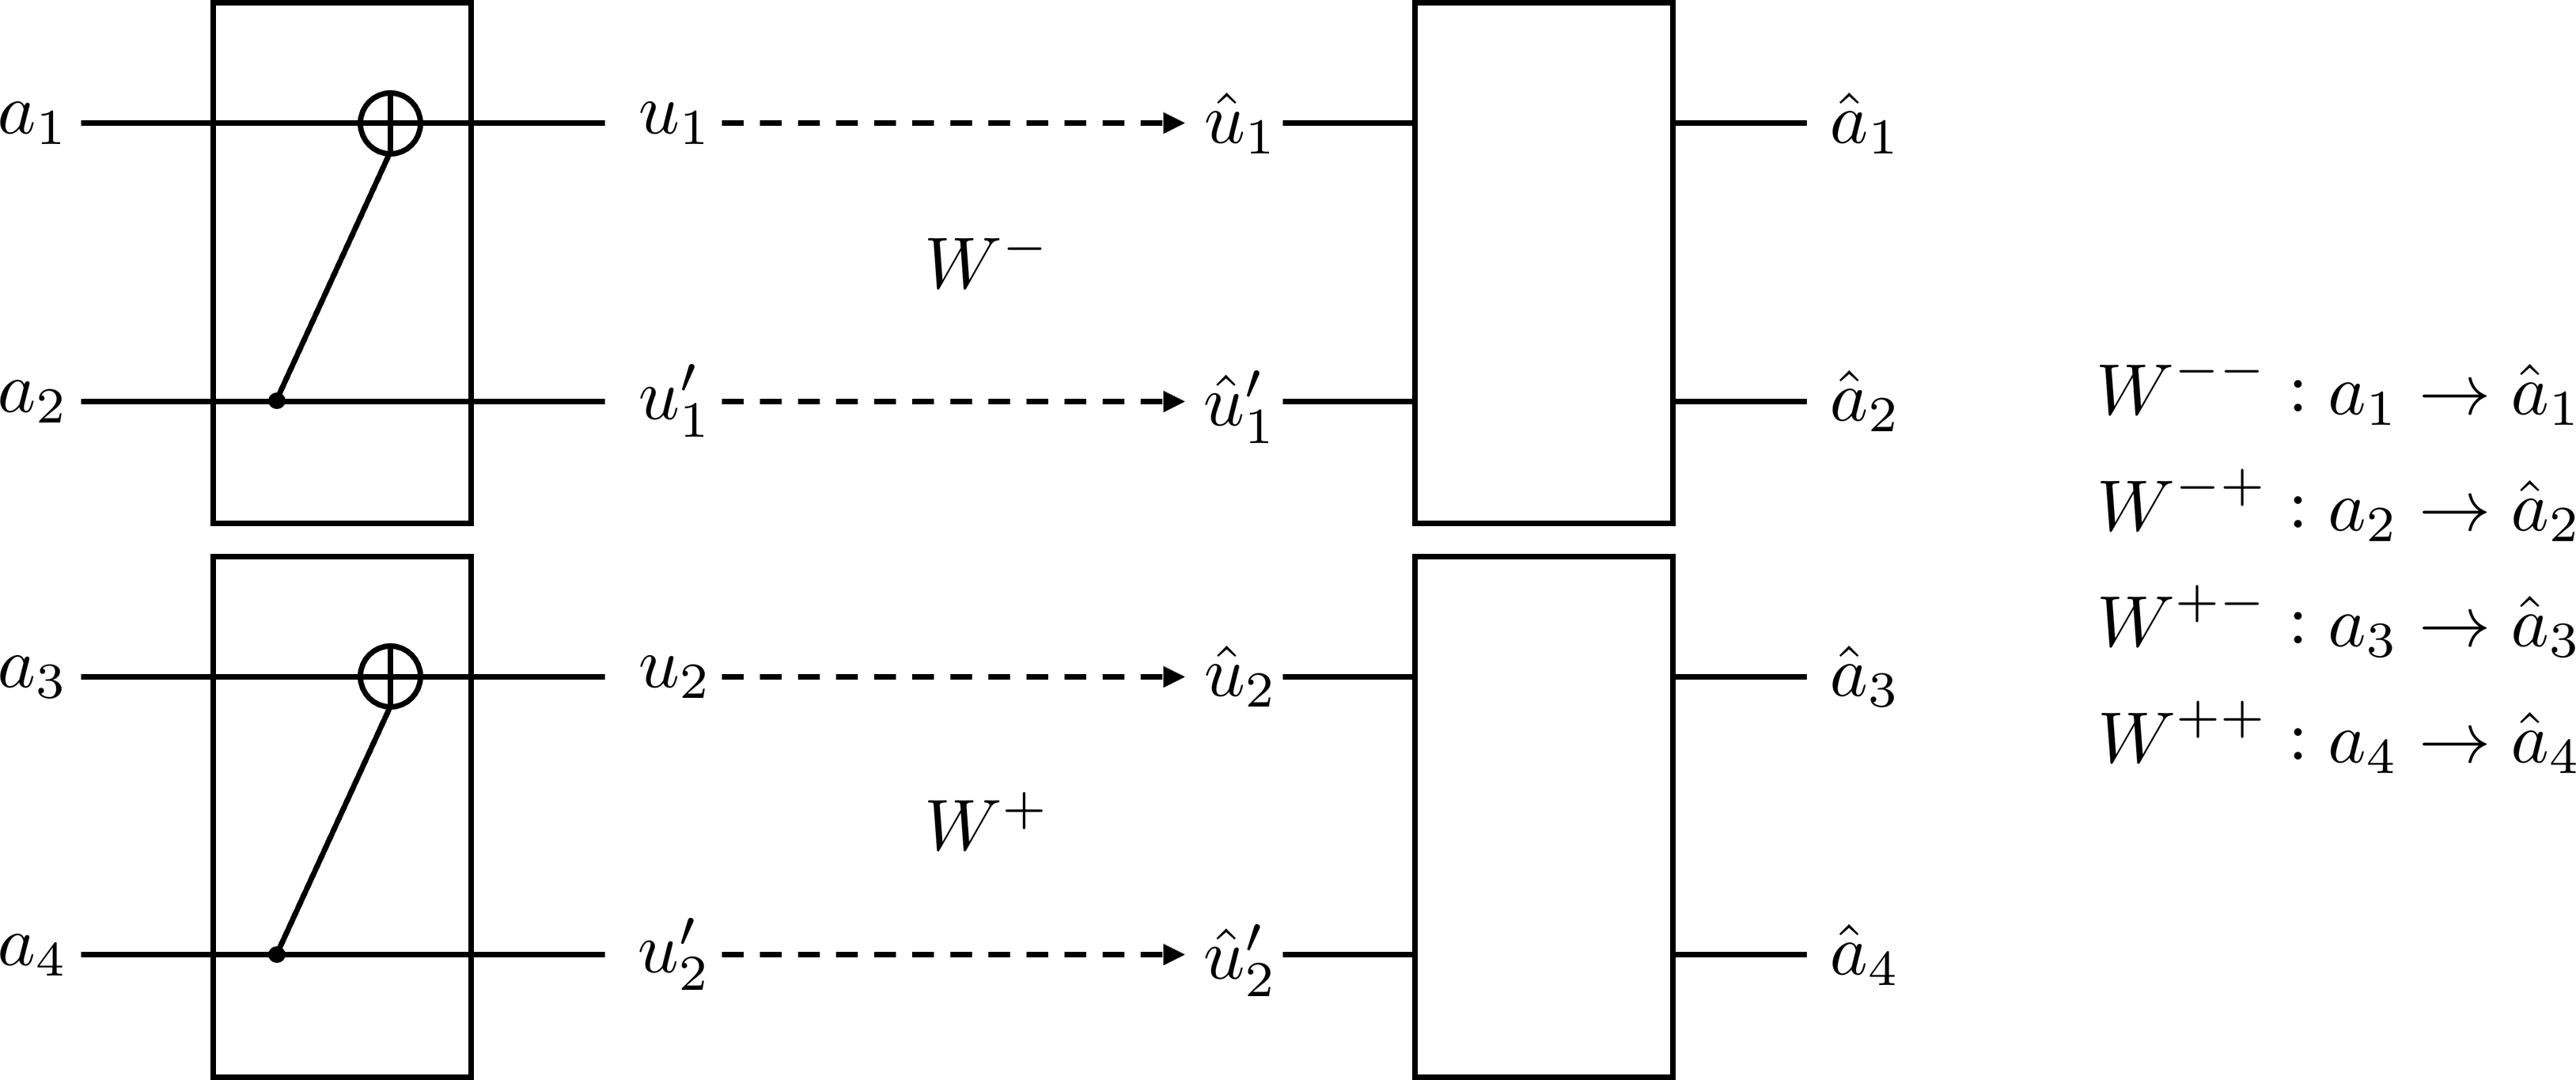
\includegraphics[width=0.8\linewidth]{w1_split_channel.png}
    \caption{Splitting channels.}
    % \label{fig:enter-label}
\end{figure}

Now we have four new sub-channels indexed by the string $s\in\{+,-\}^2$, denoting whether they are from the $+$ or the $-$ branch. The average cutoff rate thus increases further:
\begin{equation}
    R_0(W^{--}) + R_0(W^{-+}) + R_0(W^{+-}) + R_0(W^{++}) \ge 2\cdot R_0(W^{-}) + 2\cdot R_0(W^{+}) \ge 4\cdot R_0(W).
\end{equation}

\textbf{Observation}: if we repeat it indefinitely, then the average cutoff rate will continue to increase with an upper bound of $C(W)$. This bound \textit{can}, in fact, be reached:
\begin{equation}
    \frac{1}{2^n} \sum_{s\in\{+,-\}^n} R_0(W^s) \xrightarrow{n\rightarrow\infty} C(W) = \frac{1}{2^n}\sum_{s\in\{+,-\}^n} C(W^s).
\end{equation}

Amazingly, we seem to have to accept that coding at any rate under the channel capacity is ``easy.''  At this stage, Ar{\i}kan have almost invented polar code.

\section{Why ``Polar''? Asymptotic Behaviors of Polar Codes}

This section is from the paper ``Channel polarization: A method for constructing capacity-achieving codes for symmetric binary-input memoryless channels'' \cite{Channel_Polarization}. The usage of the word ``polar'' comes from the following observation:

\textbf{Observation}: For most strings $s\in\{+,-\}^n$, the values $C(W^s)$ and $R_0(W^s)$ are ``almost'' close to 0 or 1. So that the sub-channels are ``polarized.''

To wrap up, let us combine our observations above:
\begin{enumerate}
    \item $\frac{1}{2^n}\sum_{s\in\{+,-\}^n}C(W^s) = C(W)$.
    \item $C(W^s)$ is either very close to 0 or 1.
    \item The number of strings $s$ such that $C(W^s)=1$ is about $2^n C(W)$; the number of strings $s$ such that $C(W^s)=0$ is about $2^n \left(1 - C(W)\right)$.
\end{enumerate}
As a first example, let us see the easiest case of polar code over binary erasure channels. The cases for BSC, AWGN, or other general channels are harder and is considered later.

Observe that fixing an $s$ such that $C(W^s) \approx 1$, $W^s$ is such a good channel that we can transmit messages ``\textit{uncoded},'' and most of the time it transmits messages faithfully. Funnily enough, we can forget cutoff rate as a whole. We will send uncoded messages over the good sub-channels $W^s$ where $C(W^s) \approx 1$, and send deterministic bit values of 0 over the bad ones, we have the code rate as
\begin{equation}
    \text{Code rate} = \frac{\text{\# bits transmitted}}{\text{\# channel uses}=2^n} \approx C(W).
\end{equation}
Hence, polar code is capacity-achieving. All that is left is to focus on what the ``magic decoding procedures'' are from $y_i$'s to $\hat{u}_i$'s.

\begin{remark}\label{rmk:1.2}
    For $n=1$, we denote $W^{+}$ as the good sub-channel and $W^{-}$ as the bad sub-channel. Agreeing on sending 0's across the bad sub-channels ensures that we know that $\hat{u}_1$ is, and hence is good for obtaining the estimate $\hat{u}_2$ over $W^{+}$.
\end{remark}


\subsection{Binary Erasure Channel}
A binary erasure channel is a tuple represented by $(\mathcal{X},\mathcal{Y},W)$, where $\mathcal{X} = \{0,1\}$ is the input alphabet, $\mathcal{Y} = \{0,1,\mathcal{E}\}$ is the output alphabet, $\mathcal{E}$ is the erasure symbol, and
\begin{equation}
    W = \left[\begin{matrix}
        1-p & 0 & p \\
        0 & 1-p & 0
    \end{matrix}\right]
\end{equation}
is the transition matrix (see diagram below). One should be careful that in literature, the misleading notational similarity between the transition probability $W(y\vert x)$ and posterior probability $W(x|y)$ exists, one should be careful of which one is used.
\begin{figure}[H]
    \centering
    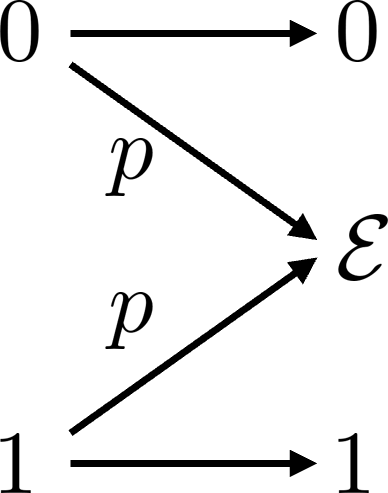
\includegraphics[width=0.1\linewidth]{w1_erasure.png}
    \caption{Illustration of a binary erasure channel.}
    % \label{fig:enter-label}
\end{figure}

A BEC is parameterized by its erasure probability $p\in[0,1]$, i.e., a BEC channel can be simply denoted uniquely as $\mathrm{BEC}(p)$.

Why do we want to use the BEC as a first example? It is due to the following two properties:
\begin{lemma}[Properties of BEC]
    \begin{enumerate}
        \item The sub-channels $\mathrm{BEC}^{+}$ and $\mathrm{BEC}^{-}$ are still BECs!
        \item We have 
        \begin{align}
            \mathrm{BEC}^{+}(x) &= \mathrm{BEC}(x^2), \label{eq:w1_bec+}\\
            \mathrm{BEC}^{-}(x) &= \mathrm{BEC}(2x-x^2). \label{eq:w1_bec-}
        \end{align}
    \end{enumerate}
\end{lemma}

\begin{lemma}[Channel Capacity of BEC]
    \begin{equation}
        C\left(\mathrm{BEC}(x)\right) = 1-x
    \end{equation}
\end{lemma}

\begin{proof}
    Let $X\sim \mathrm{Ber}(\alpha)$, then the mutual information will be
    \begin{align*}
        I(X;Y) &= H(Y) - H(Y|X) \\
        % &= -\left[\alpha(1-p) \lg\alpha(1-p) + (1-\alpha)(1-p) \lg(1-\alpha)(1-p) + p \lg p\right] \\
        % &\;\;\;\;\;+ \left[\alpha \cdot \left(p\lg p + (1-p)\lg(1-p)\right) + (1-\alpha) \cdot \left(p\lg p + (1-p)\lg(1-p)\right)\right] \\
        &= -\alpha(1-p) \lg\alpha(1-p) - (1-\alpha)(1-p) \lg(1-\alpha)(1-p) + (1-p)\lg(1-p).
    \end{align*}
    The maximum is achieved at
    \begin{align*}
        \diff{}{\alpha} I(X;Y) = 0 &= -(1-p)\left(\lg\alpha(1-p) + 1\right) + (1-p)\left(\lg(1-\alpha)(1-p) + 1\right) \\
        &\rightarrow \lg\alpha = \lg(1-\alpha) \rightarrow \alpha = \frac{1}{2}.
    \end{align*}
    Hence the channel capacity is
    \begin{align*}
        C\left(\mathrm{BEC}(p)\right) = \left.I(X;Y)\right|_{\alpha=\frac{1}{2}} = -(1-p)\lg\frac{1-p}{2} + (1-p) \lg (1-p) = (1-p).
    \end{align*}
    Thus it is proven.
\end{proof}

From the above lemmas, we can check that BEC satisfies our previous observation:
\begin{equation*}
    C\left(\mathrm{BEC}(p)^{+}\right) + C\left(\mathrm{BEC}(p)^{-}\right) = (1-x^2) + (1-2x+x^2) = 2-2x = 2\cdot C\left(\mathrm{BEC}(p)\right).
\end{equation*}
Further, for the $+$ channels, the erasure probability reduces to $x^2$, while for the $-$ channels, the erasure probability increases to $1-(1-x)^2$. The $+$ channels quickly become faithful as their erasure probability $p\rightarrow 0$, while the $-$ channels quickly become useless as $p\rightarrow1$. A quantitative description is as follows:
\begin{theorem}[Speed of Polarization] \label{thm:w1_polar_speed}
    There exists a function $f:[0,1] \rightarrow [0,1]$ that has shape quite similar to $[x(1-x)]^{0.7}$ satisfying the following functional equation:
    \begin{equation}\label{eq:w1_speed_of_polarization_1}
        \frac{f(x^2) + f(2x-x^2)}{2f(x)} \approx 2^{-\frac{1}{3.627}} \approx 0.826.
    \end{equation}
    Consequently,
    \begin{equation}\label{eq:w1_speed_of_polarization_2}
        \frac{1}{2^nf(x)} \sum_{s\in\{+,-\}^n} f\left(\text{erasure probability of }\mathrm{BEC}(x)^s\right) \approx 2^{-\frac{n}{3.627}} \approx 0.826^n.
    \end{equation}
\end{theorem}
Since the RHS of the above equation is small, most of ``$f\left(\text{erasure probability of }\mathrm{BEC}(x)^s\right)$'' is small as well. Looking at the graph of $f\approx[x(1-x)]^{0.7}$, we see that $x$ must be close to 0 or 1. Henceforth, $\mathrm{BEC}^s(x)$ is mostly equal to either $\mathrm{BEC}(0)$ or $\mathrm{BEC}(1)$. What's more, the theorem above states that the quantitative speed of channel polarization is exponential in the order of $2^{-\frac{n}{3.627}}$. For general channels, we have the speed of polarization in the order of $2^{-\frac{n}{4}}$, with a mathematically rigorous bound currently at $2^{-\frac{n}{4.71\cdots}}$. Moreover, the derivation from \autoref{eq:w1_speed_of_polarization_1} to \autoref{eq:w1_speed_of_polarization_2} is as follows:
\begin{proof}
    Assume such $f$ exists, then plugging in $x^2$ and $2x-x^2$, we obtain
    \begin{equation*}
    \begin{cases}
        f(x^4) + f(2x^2-x^4) = 2^{-\frac{1}{3.627}}\cdot 2 f(x^2) \\
        f((2x-x^2)^2) + f(2(2x-x^2)-(2x-x^2)^2) = 2^{-\frac{1}{3.627}}\cdot 2 f(2x-x^2)
    \end{cases}.
    \end{equation*}
    Then, we have
    \begin{align*}
        f(x^4) + f(2x^2-x^4) &+ f((2x-x^2)^2) + f(2(2x-x^2)-(2x-x^2)^2) \\
        &= 2^{-\frac{1}{3.627}}\cdot2\left(f(x^2) + f(2x-x^2)\right) = 2^{-\frac{2}{3.627}}\cdot 4f(x).
    \end{align*}
    Continue on this trend, we will obtain \autoref{eq:w1_speed_of_polarization_2} by induction.
\end{proof}
\autoref{eq:w1_speed_of_polarization_1} is sort of like an eigenvalue problem, with $f$ as the eigenfunction and $2^{-\frac{1}{3.627}}$ as the eigenvalue. As of when this script was written, the only method for proving and showing speed of polarization is using the above ``power-sum method'' or some other similar variants. For more details, also refer to the paper ``On the rate of channel polarization'' \cite{On_the_Rate_of_Channel_Polarization}.

If the erasure probability $x$ is very small, say $2^{-20}$, then $x^2 = 2^{-40}$ and $2x - x^2 \approx 2^{-19}$. We can approximate the sub-channels as
\begin{equation}
    \mathrm{BEC}(x)^s \approx \mathrm{BEC}(x^{\overbrace{2\times\cdots\times 2}^{\text{\# of $+$'s in $s$}}}).
\end{equation}

Then, for arbitrary $s\in\{+,-\}^n$, as a conservative bound we have about $n(\frac{1}{2}-\varepsilon)$ of $+$'s in $s$ with high probability. Then if $x$ is small, then most $\mathrm{BEC}(x)^s \approx \mathrm{BEC}(x^{2^{n/2}})$. Further recall that the amount of strings $s$ such that $\mathrm{BEC}(x)^s$ has small erasure probability is $2^n C\left(\mathrm{BEC}(x)\right)$. Now we know that not only are a fraction (approximately $C(W)$) of $W^s$'s are good, but they are also approximately $\mathrm{BEC}(x^{2^{n/2}})$-good, i.e., we have good channels that are ``exponentially exponentially decaying!''

% \section{Agenda}
The agenda for this course will hence be to prove the \textit{observations} and facts listed above. Further, we will also discuss generalizations of polar codes: BEC, BSC, AWGN, asymmetric channels, deletion channels, Markovian channels, non-stationary channels, source coding, rate distortion, wiretap, broadcast, multiple access channels, larger alphabet, larger kernel, $\ldots$.


\section{The Big Picture}
There is a correspondence between probability theory and coding theory:

\begin{table}[H]
    \centering
    \begin{tabularx}{\textwidth}{X|X|X}
        \multicolumn{1}{c}{Probability Theory} & \multicolumn{1}{c}{Random Codes} & \multicolumn{1}{c}{Polar Codes} \\ \hline\hline
        For i.i.d. $X_1,\ldots,X_N$, we have the \textit{concentration inequality}:
        \resizebox{\linewidth}{!}{
        $\begin{aligned}
            \mathrm{Pr}\left\{\frac{X_1+\cdots+X_N}{N} -\mathbb{E}[X_1] \ge t\right\} \\ \le \exp(-ct^2N)
        \end{aligned}$
        }
        for some constant $c$. This is also known as the \textit{large deviation principle / behavior}, it can be derived from Hoeffding's inequality. &
        Over a channel $W$ with fix rate $R<C(W)=C$, let the block length be $N$. Then there exists a good code of block error probability
        \begin{equation*}
            \approx \exp(-c(C-R)^2N)
        \end{equation*}
        for some constant $C$. &
        At block length $N$, code rate $R<C$, the bound for error probability is $\approx\exp(-\sqrt{N})$ for polar code, and can be improved to $\approx\exp(-N^{0.9})$ for other schemes.\\ \hline
        The central limit theorem (CLT) states that
        \resizebox{\linewidth}{!}{
        $\begin{aligned}
            Z \defeq \frac{X_1+\cdots+X_N}{\sqrt{N}} - \sqrt{N}\mu \\ \sim \mathcal{N}(0,\sigma^2),
        \end{aligned}$
        }
        where $\mu=\mathbb{E}[X_1]$ and $\sigma^2=\mathrm{Var}(X_1)$. This is also known as the \textit{small deviation principle}. & 
        At block length $N$, and fix $p$ as block error probability. The code rate is
        \begin{equation*}
            R \approx C- O\left(\frac{1}{\sqrt{N}}\right).
        \end{equation*} &
        At block length $N$, and fix $p$ as block error probability. The code rate is
        \begin{equation*}
            R\approx C-O(N^{-1/3.6})
        \end{equation*}
        for polar code, and the exponent can be improved to $N^{-1/2.1}$. \\ \hline
        The \textit{moderate deviation principle} asks what is the distribution that the following R.V. follows?
        \begin{equation*}
            Y \defeq \frac{X_1+\cdots+X_N}{N^\alpha}-\frac{N\mu}{N^\alpha}
        \end{equation*} &
        There is a tradeoff between $R$ and $p$. &
        There is a tradeoff between $R$ and $p$.
    \end{tabularx}
    % \caption{Caption}
    % \label{tab:my_label}
\end{table}
As a side note, if the polar code is $n$-layer deep, then the block length $N=2^n$.

This big picture is what one should keep in mind throughout this lecture note. Further note that the results for coding theory are often proved using random coding, which is not really practical. Hence, we also provided the bounds for practical codes such as the polar codes in the table above.

% \begin{remark}[Block Length]
%     In case one forgot, the block length $N$ of a code is the number of bits in a block. It is related to the number $n$ defined in \autoref{sec:w1_origin_of_polar_code} by $N=2^n$.
% \end{remark}

% The relation between small, moderate, and large deviation behaviors are also seen in source coding and hypothesis testing. See the lecture slides by prof. Hao-Chung Cheng on Quantum Compression, Classical Communication in the course Quantium Information and Computation for nice illustrations and more information. An excerpt from the source coding theory is shown in the figure below:
% \begin{figure}[H]
%     \centering
%     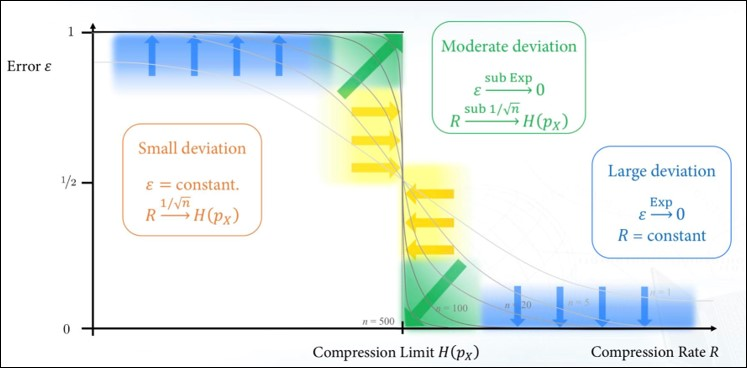
\includegraphics[width=0.8\linewidth]{figures/w1_deviation.jpg}
% \end{figure}

